\documentclass{ximera}
\usepackage{tikz}
\usetikzlibrary{shapes.geometric, arrows}

\tikzstyle{startstop} = [rectangle, rounded corners, minimum width=3cm, minimum height=1cm, text centered, fill=red!50]
\tikzstyle{io} = [trapezium, trapezium left angle=70, trapezium right angle=110, minimum height=1cm, text centered, fill=blue!30]
\tikzstyle{process} = [rectangle, minimum width=3cm, minimum height=1cm, text centered, text width=3cm, fill=orange!50]
\tikzstyle{decision} = [diamond, minimum width=3cm, minimum height=1cm, text centered, text width=2cm, fill=green!30]
\tikzstyle{arrow} = [thick,->,>=stealth]

\title{Newton's Method}
\begin{document}
\begin{abstract}
We give an introduction to finding roots using Newton's Method.
\end{abstract}
\maketitle

\section{Linear Approximations}

In a calculus course, it is shown that the best linear approximation to a differentiable function $f(x)$ near $x=a$ is given by $L_a(x)=f'(a)(x-a)+f(a)$. We will make use of this general idea to try to approximate solutions of equations of the form $f(x)=0$.

The Desmos interactive graph below gives an example of a linear approximation to a differentiable function.

\desmos{adu2uowy3n}{800}{600}

\section{Newton's Method}

Suppose that $f(x)$ is a differentiable function and that we would like to solve the equation $f(x)=0$. Using the IVT, or a graphical method, we might have an initial guess for a solution that we will call $x_0$. We are interested in finding a value $r$ such that $f(r)=0$. We know that if $r$ and $x_0$ are ``close" to each other, then $$f(r)\approx f'(x_0)(r-x_0)+f(x_0).$$ Setting the right-hand side above equal to 0, solving for $r$ in terms of $x_0$, and renaming $r$ as $x_1$ gives that $$x_1=x_0-\frac{f(x_0)}{f'(x_0)}.$$ Iterating this process gives that $$x_n=x_{n-1}-\frac{f(x_{n-1})}{f'(x_{n-1})}$$ for $n\geq 1$. We can iterate the above procedure until $|f(x_n)|$ becomes as small as we like, at which point the claim is that $x_n$ is an approximate solution to the equation.

The Desmos interactive graph below gives an example of Newton's method iterated twice.

\desmos{zokv8syqrv}{800}{600}

Before we go over the algorithm for Newton's Method, we must note a disadvantage of this method. Unlike the Binomial Method, Newton's Method may not converge (try applying the method to $f(x)=x^{1/3}$). We must therefore specify a maximum number of iterations we are willing to compute to ensure that the algorithm terminates.

We can summarize Newton's Method using the following flowchart. Here we assume that $f(x)$ is differentiable, that $f'(x)\neq 0$, that $x_0$ is close to a solution of $f(x)=0$, that $n$ is the maximum number of iterations we are willing to compute, and that $err>0$.

\begin{center}
    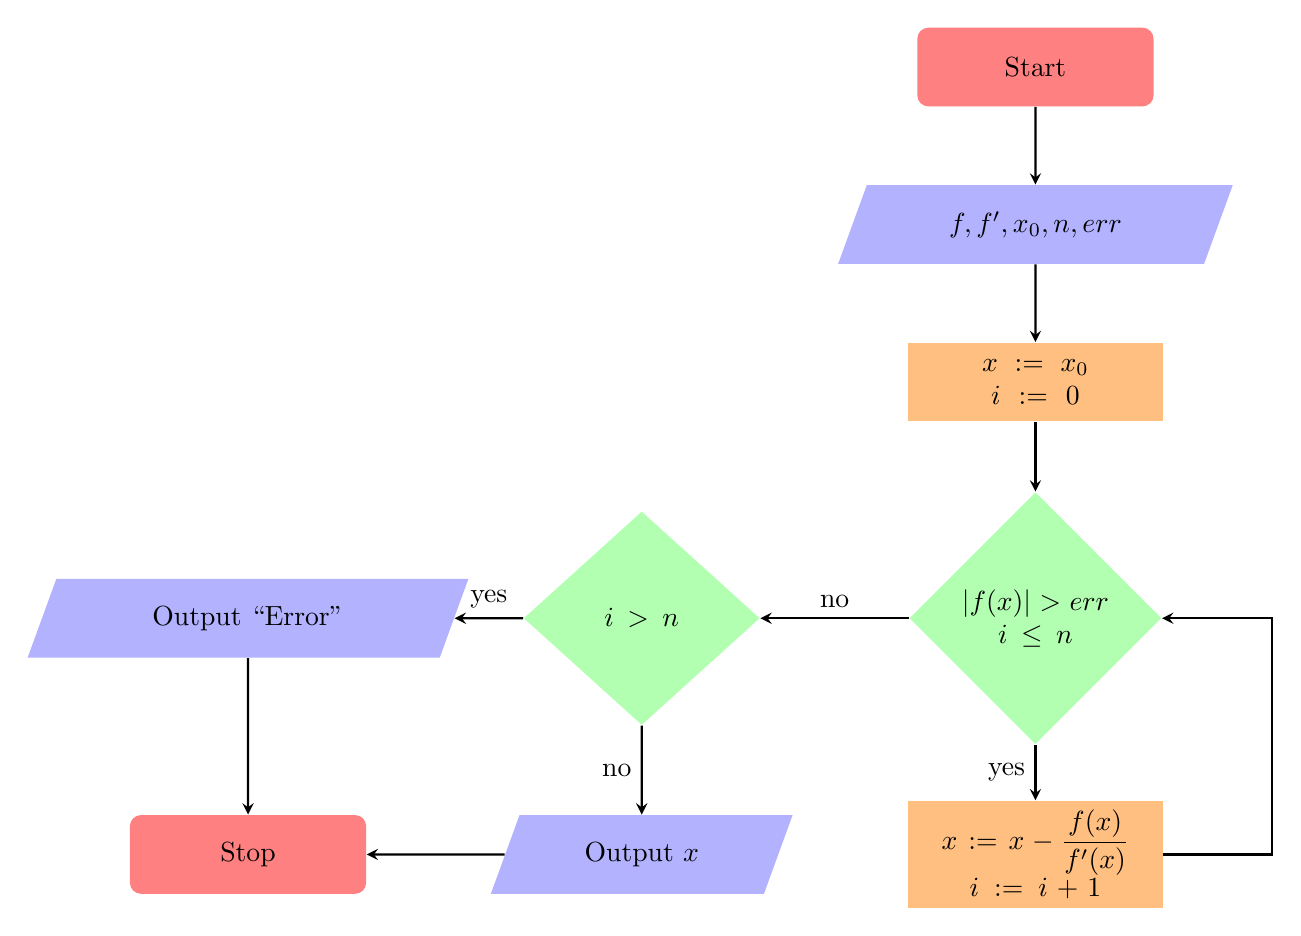
\begin{tikzpicture}
    \node [startstop] at (0,0) (start) {Start};
    \node [io] at (0,-2) (io1) {$f,f',x_0,n,err$};
    \node [process] at (0,-4) (process1) {$x:=x_0$\\$i:=0$};
    \node [decision] at (0,-7) (decision1) {$|f(x)|>err$\\$i\leq n$};
    \node [decision] at (-5,-7) (decision2) {$i>n$};
    \node [process] at (0,-10) (process2) {$x:=x-\displaystyle\frac{f(x)}{f'(x)}$\\$i:=i+1$};
    \node [io] at (-5,-10) (io2) {Output $x$};
    \node [io] at (-10,-7) (io3) {Output ``Error"};
    \node [startstop] at (-10,-10) (stop) {Stop};

    \draw [arrow] (start) -- (io1);
    \draw [arrow] (io1) -- (process1);
    \draw [arrow] (process1) -- (decision1);
    \draw [arrow] (decision1) -- node[anchor=east] {yes} (process2);
    \draw [arrow] (decision1) -- node[anchor=south] {no} (decision2);
    \draw [arrow] (decision2) -- node[anchor=east] {no} (io2);
    \draw [arrow] (decision2) -- node[anchor=south] {yes} (io3);
    \draw [arrow] (process2) -- (3,-10) |- (decision1);
    \draw [arrow] (io2) -- (stop);
    \draw [arrow] (io3) -- (stop);
    \end{tikzpicture}
\end{center}

Converting this flowchart to code gives the following:

\begin{verbatim}
==============================
def newton(f,df,x0,n,error):
        x = x0
        i = 0
        while abs(f(x)) > error and i <= n:
                x = x - f(x)/df(x)
                i += 1
        if i > n:
                return "Exceeded iterations"
        else:
                return x
==============================
\end{verbatim}

While Newton's Method may fail to converge, one advantage of this method is that it converges to a solution faster than the Binomial Method in many cases.

\section{Problems}

All answers in this section have been rounded to the nearest thousandth, the error for the output has been set to $0.0001$, and the number of iterations have been capped at 10.

\begin{question}
	Use Newton's Method to estimate the solution to $f(x)=0$ where $f(x)=x^3-5$. $\answer{1.710}$
\end{question}

\begin{question}
	Use the Newton's Method to give an approximation of $\sqrt{3}$. $\answer{1.732}$
\end{question}

\begin{question}
	Use Newton's Method to give an approximation of the solutions to the equation $x\ln^2{x}=1/2$. Enter your solutions in incresing order. $\answer{0.073}$ $\answer{0.226}$ $\answer{1.716}$
	\begin{hint}
	Different initial values will converge to different solutions. Use a graphical method to determine different initial values.
	\end{hint}
\end{question}

\section{Workspace}

\begin{sageCell}
# Use this cell to solve the above questions.
\end{sageCell}

\end{document}
